\documentclass{beamer}
\usetheme{Boadilla}
\usepackage[utf8]{inputenc}

\usetheme{Madrid}
\usepackage[version=3]{mhchem}
\usepackage{hepunits}
\usepackage{eurosym}

\usepackage{multicol} %%Multicolumns

\setbeamertemplate{navigation symbols}{} 
\useoutertheme{infolines}

\title[TRITIUM-IFIC 2]{Results of TRITIUM-IFIC 2 prototypes}
\author[M. Martinez-Roig]{Marcos Martinez Roig}
\institute[IFIC]{Instituto de Física Corpuscular, Valencia, España}
\date[15/10/2020]{15/10/2020}

\begin{document}

\begin{frame}
\titlepage
\end{frame}

\begin{frame}
\frametitle{Outline}
\tableofcontents
\end{frame}

\section{Tritium-IFIC 2}
\begin{frame}
\frametitle{Tritium-IFIC 2 Prototype}

\begin{multicols}{2}

\begin{figure}[hbtp]
\centering
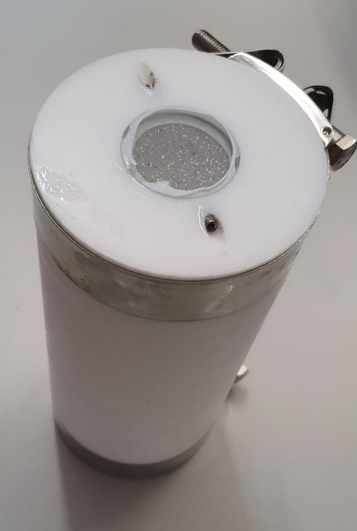
\includegraphics[scale=0.3]{Imagenes/1Tritium_detector/Tritium_Lab_Prototype.png}
\caption{TRITIUM-IFIC 2, laboratory prototype}
\end{figure}

\columnbreak

\begin{figure}[hbtp]
\centering
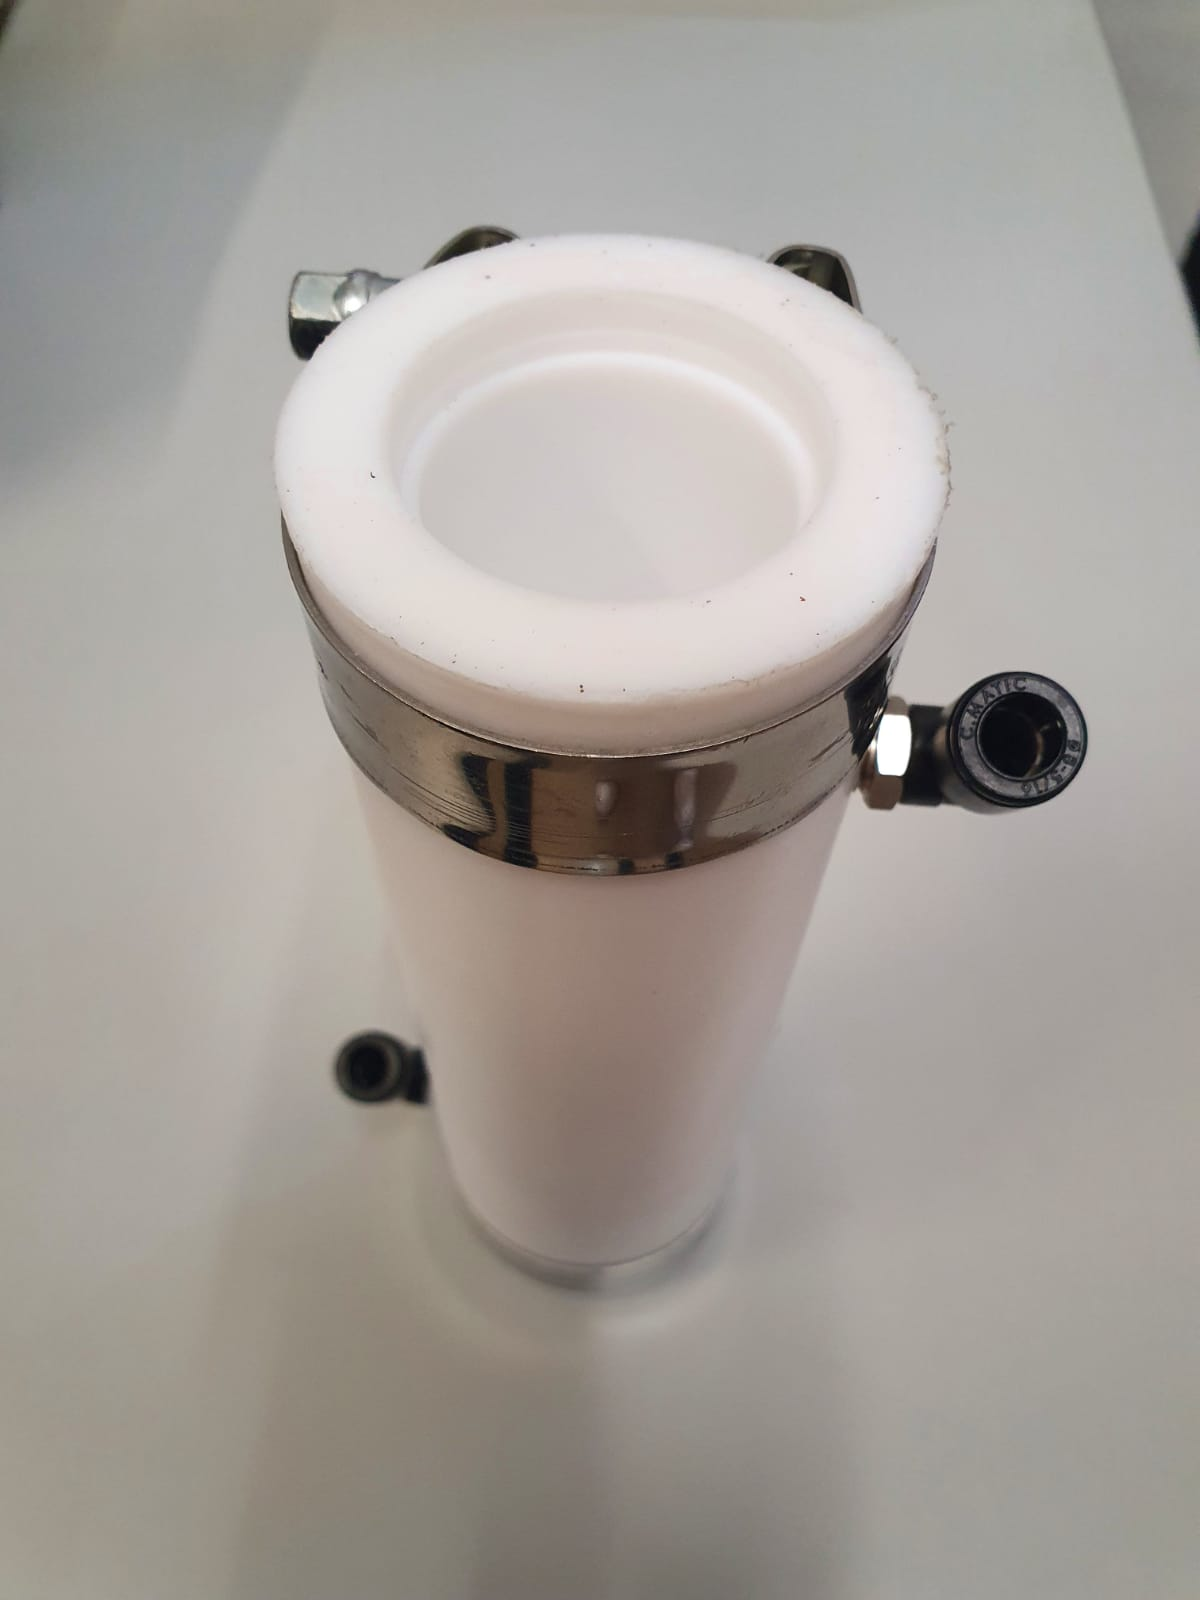
\includegraphics[scale=0.1]{Imagenes/1Tritium_detector/Tritium_Arrocampo_Prototype.jpeg}
\caption{TRITIUM-IFIC 2, Arrocampo cell}
\end{figure}

\end{multicols}

\end{frame}

\begin{frame}
\frametitle{Tritium-IFIC 2 (Prototypes + Cosmic Vetos)}

FOTOOS PROTOTIPO CON VETOS

\end{frame}

\begin{frame}
\frametitle{Tritium-IFIC 2 read-out electronic system}

\begin{figure}[hbtp]
\centering
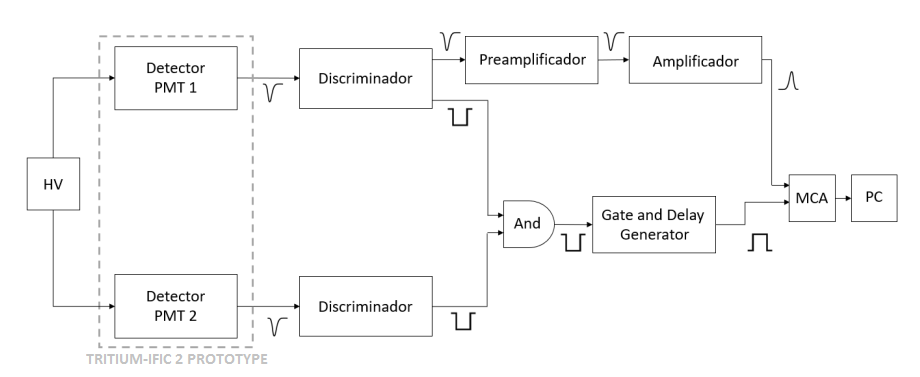
\includegraphics[scale=0.5]{Imagenes/1Tritium_detector/Esquema_electronico.png}
\caption{Scheme of the read-out electronic system}
\end{figure}

\end{frame}

\begin{frame}
\frametitle{Tritium-IFIC 2 read-out electronic system}

\begin{figure}[hbtp]
\centering
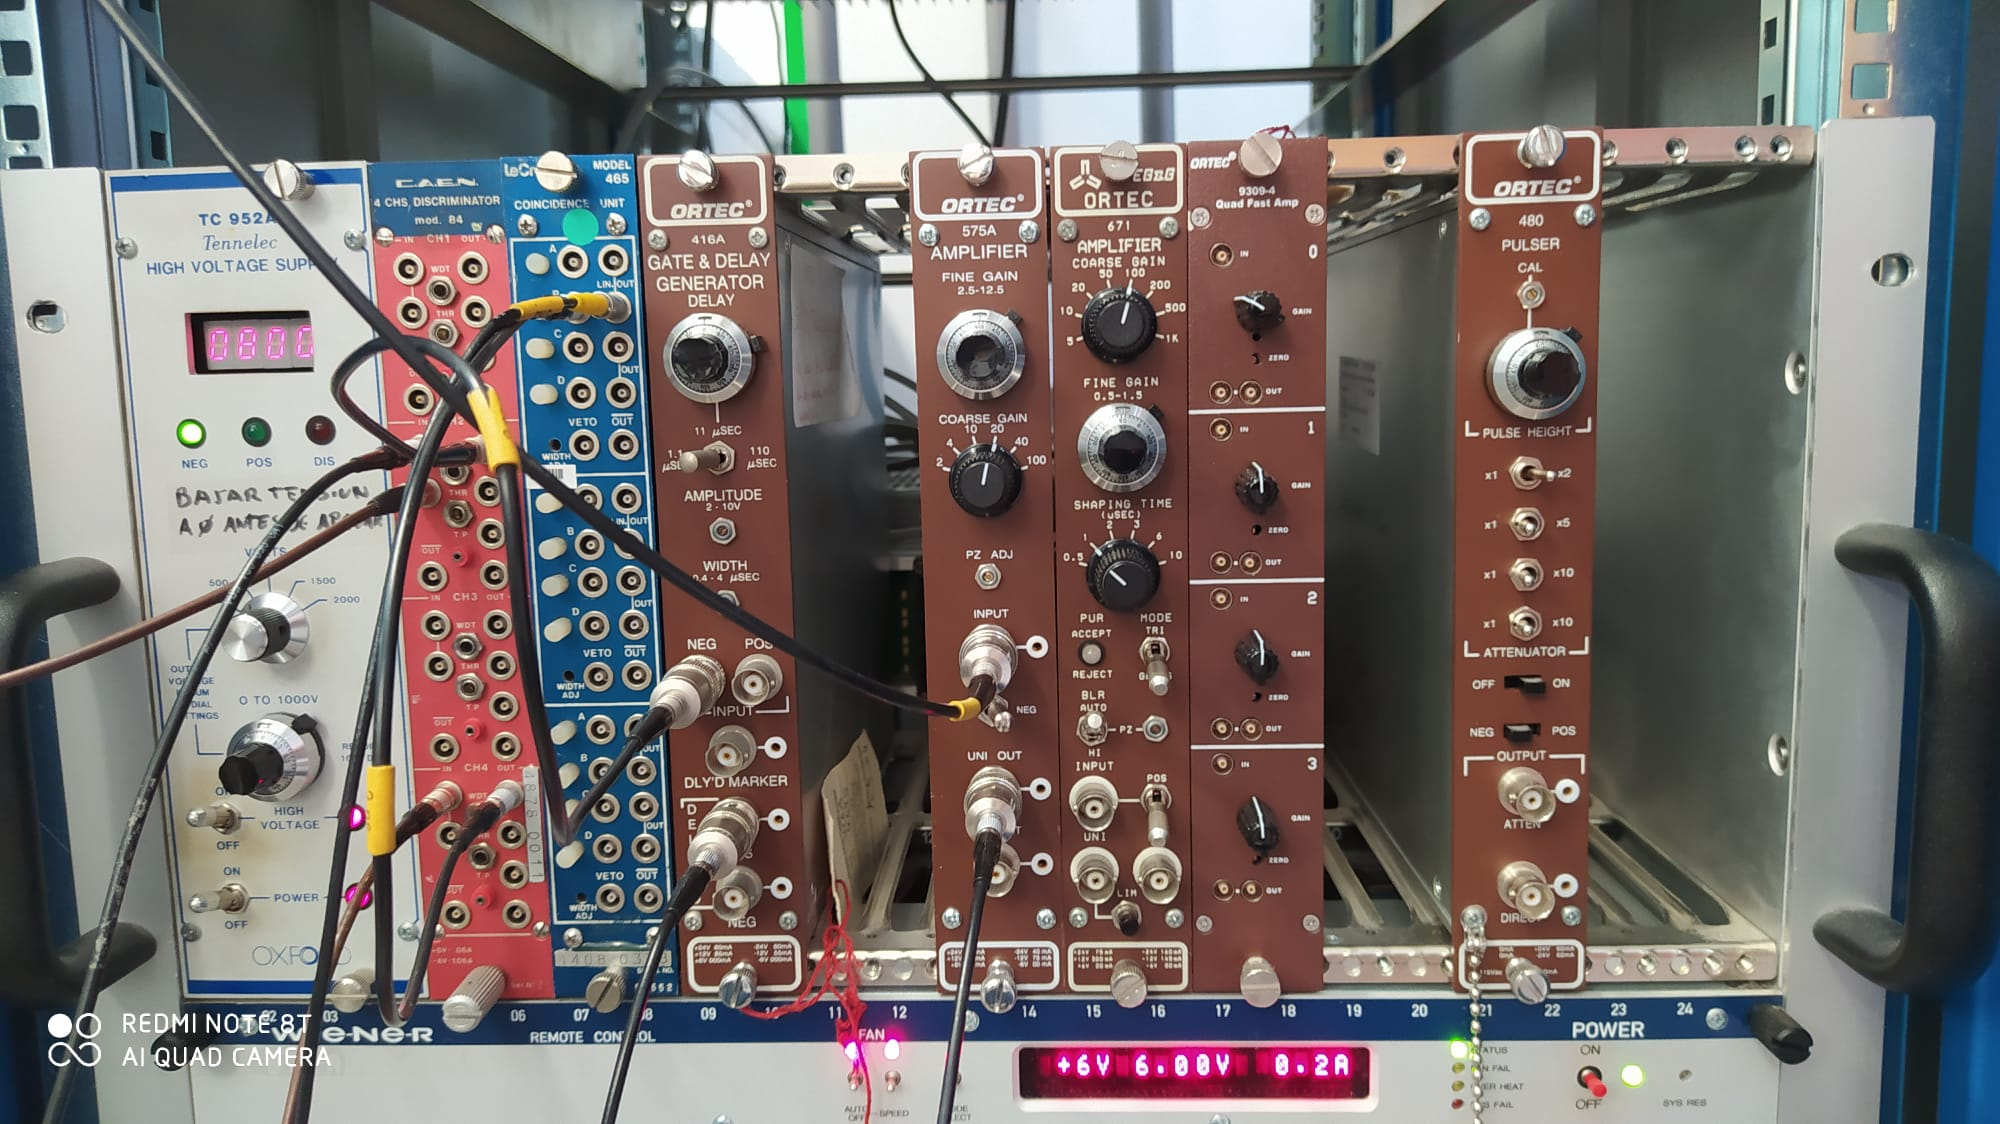
\includegraphics[scale=0.16]{Imagenes/1Tritium_detector/Sistema_electronico.jpeg}
\caption{Read-out electronic system}
\end{figure}

\end{frame}

\section{Prototype efficiency measurement}
\begin{frame}
\frametitle{Prototype efficiency measurement}

\begin{table}
\begin{tabular}{l | c}
Parameter & Numerical value\\
\hline \hline
Number of fibers in each prototypes & $800$ \\
Distance of fibers in each prototypes& $20~\cm$ \\
Diameter of the fibers in each prototype & $1~\mm$ \\
Activity of tritium solution & $10~\kilo\becquerel/\liter$ \\
Date (signal) & 20/07/2020 \\
Air conditioned (signal) & ON ($18~\degree$) \\
Fans inside the black box (signal) & ON \\
Date (background) & 22/05/2020 \\
Air conditioned (background) & ON ($18~\degree$) \\
Fans inside the balck box (background) & ON \\
Low Level discrimination channel (MCA) & $100\approx 122$ mV \\
\end{tabular}

\caption{Relevant information for the measurement}
\end{table}

\end{frame}


\begin{frame}
\frametitle{Prototype efficiency measurement}

\begin{figure}[hbtp]
\centering
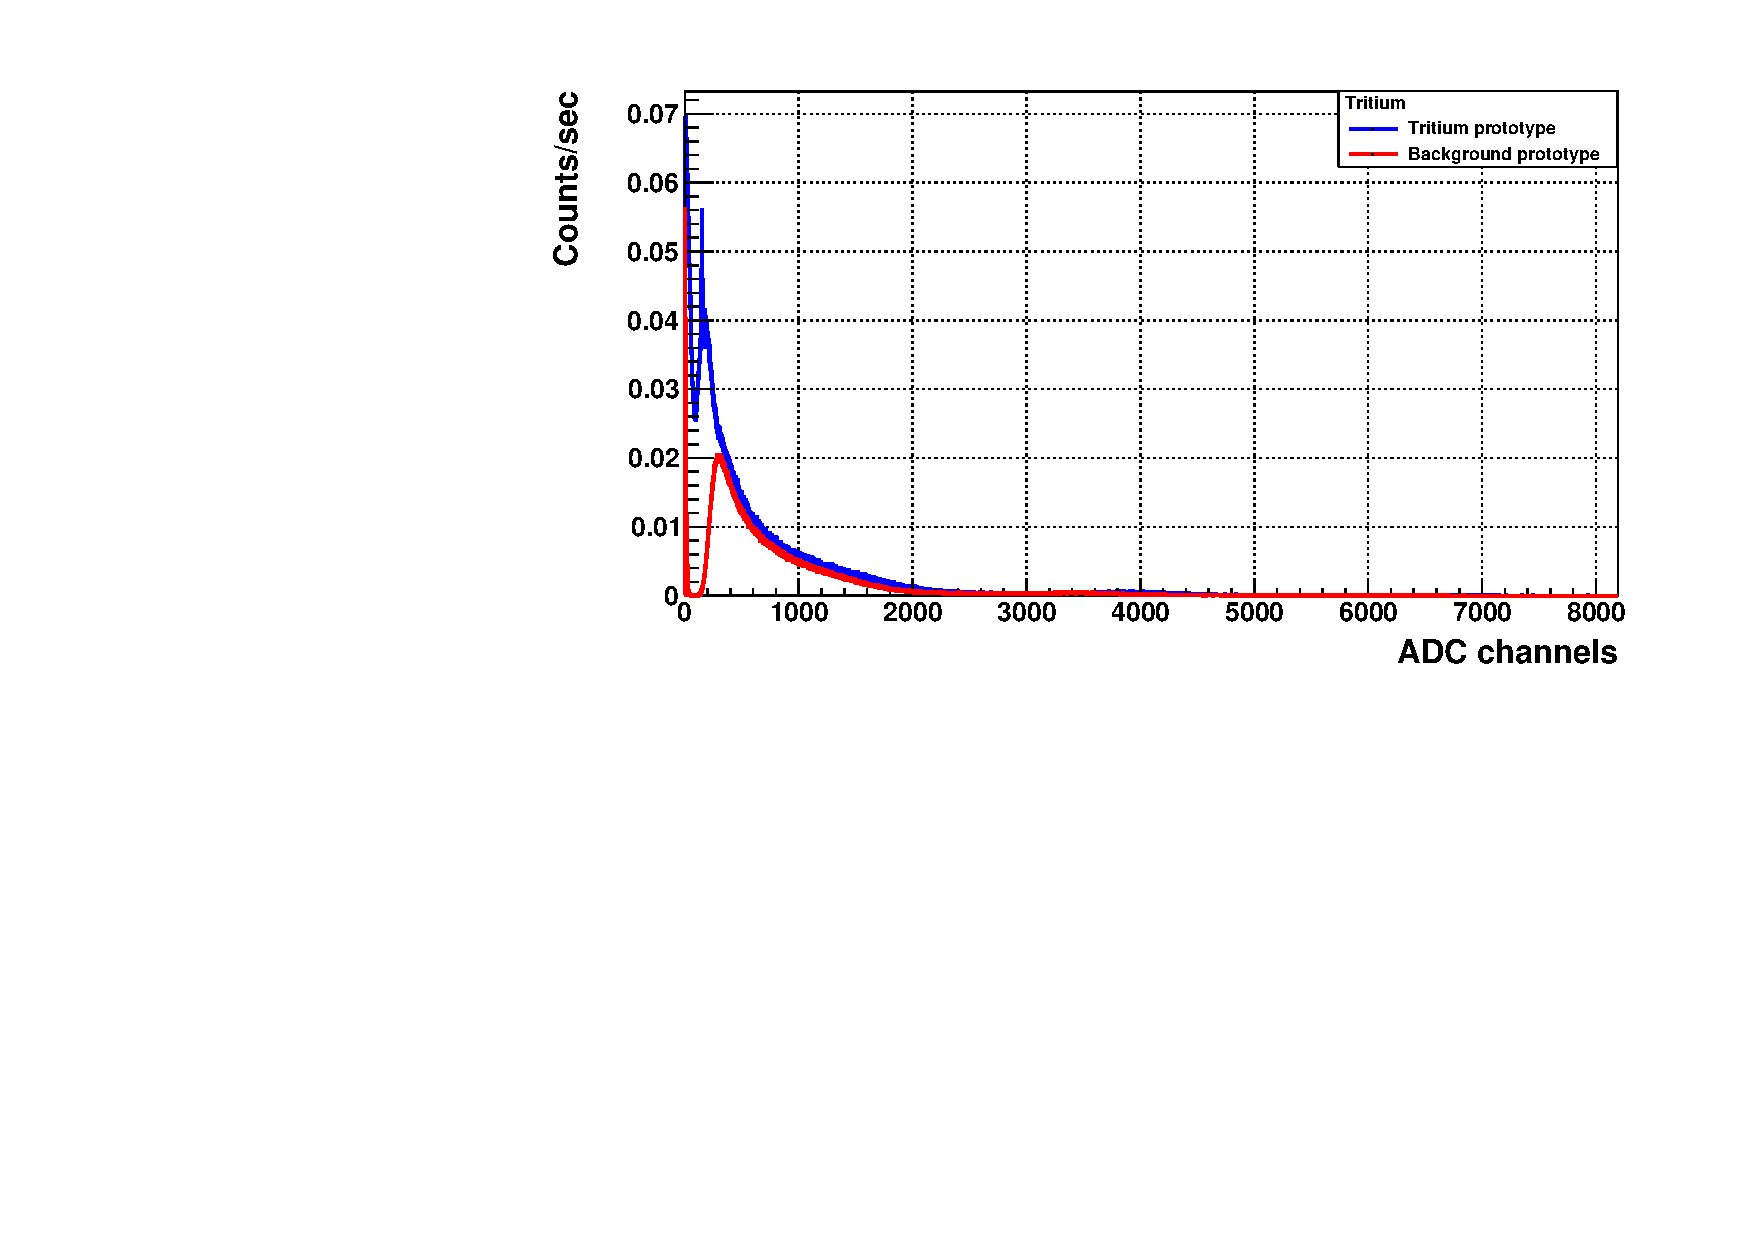
\includegraphics[scale=0.6]{Imagenes/2Efficiency/Signal_background_real_time.pdf}
\caption{Signals of both TRITIUM-IFIC 2 prototypes}
\end{figure}


\end{frame}

\begin{frame}
\frametitle{Prototype efficiency measurement}

\begin{figure}[hbtp]
\centering
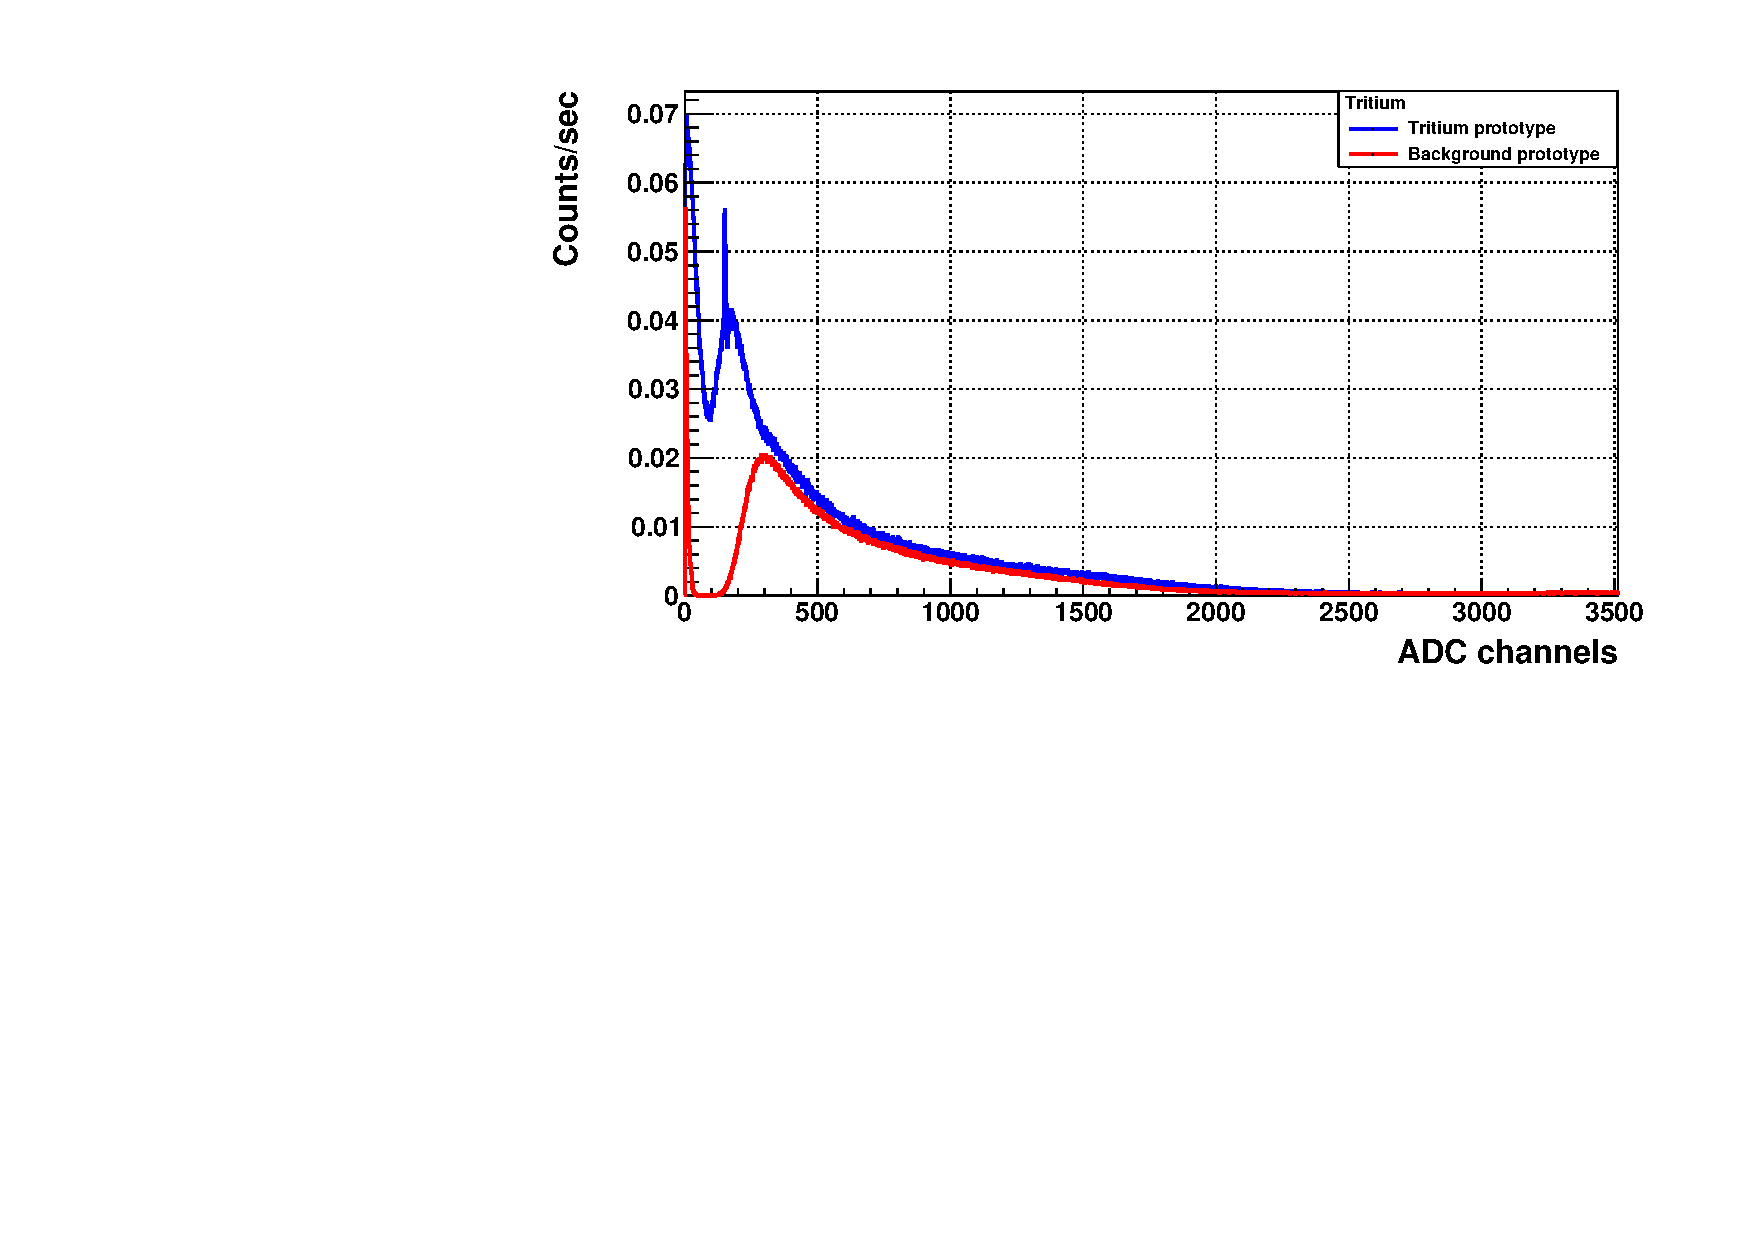
\includegraphics[scale=0.6]{Imagenes/2Efficiency/Signal_background_real_time_ZOOM.pdf}
\caption{Signals of both TRITIUM-IFIC 2 prototypes (Zoom 0-4000 channels)}
\end{figure}


\end{frame}

\begin{frame}
\frametitle{Prototype efficiency measurement}

\begin{figure}[hbtp]
\centering
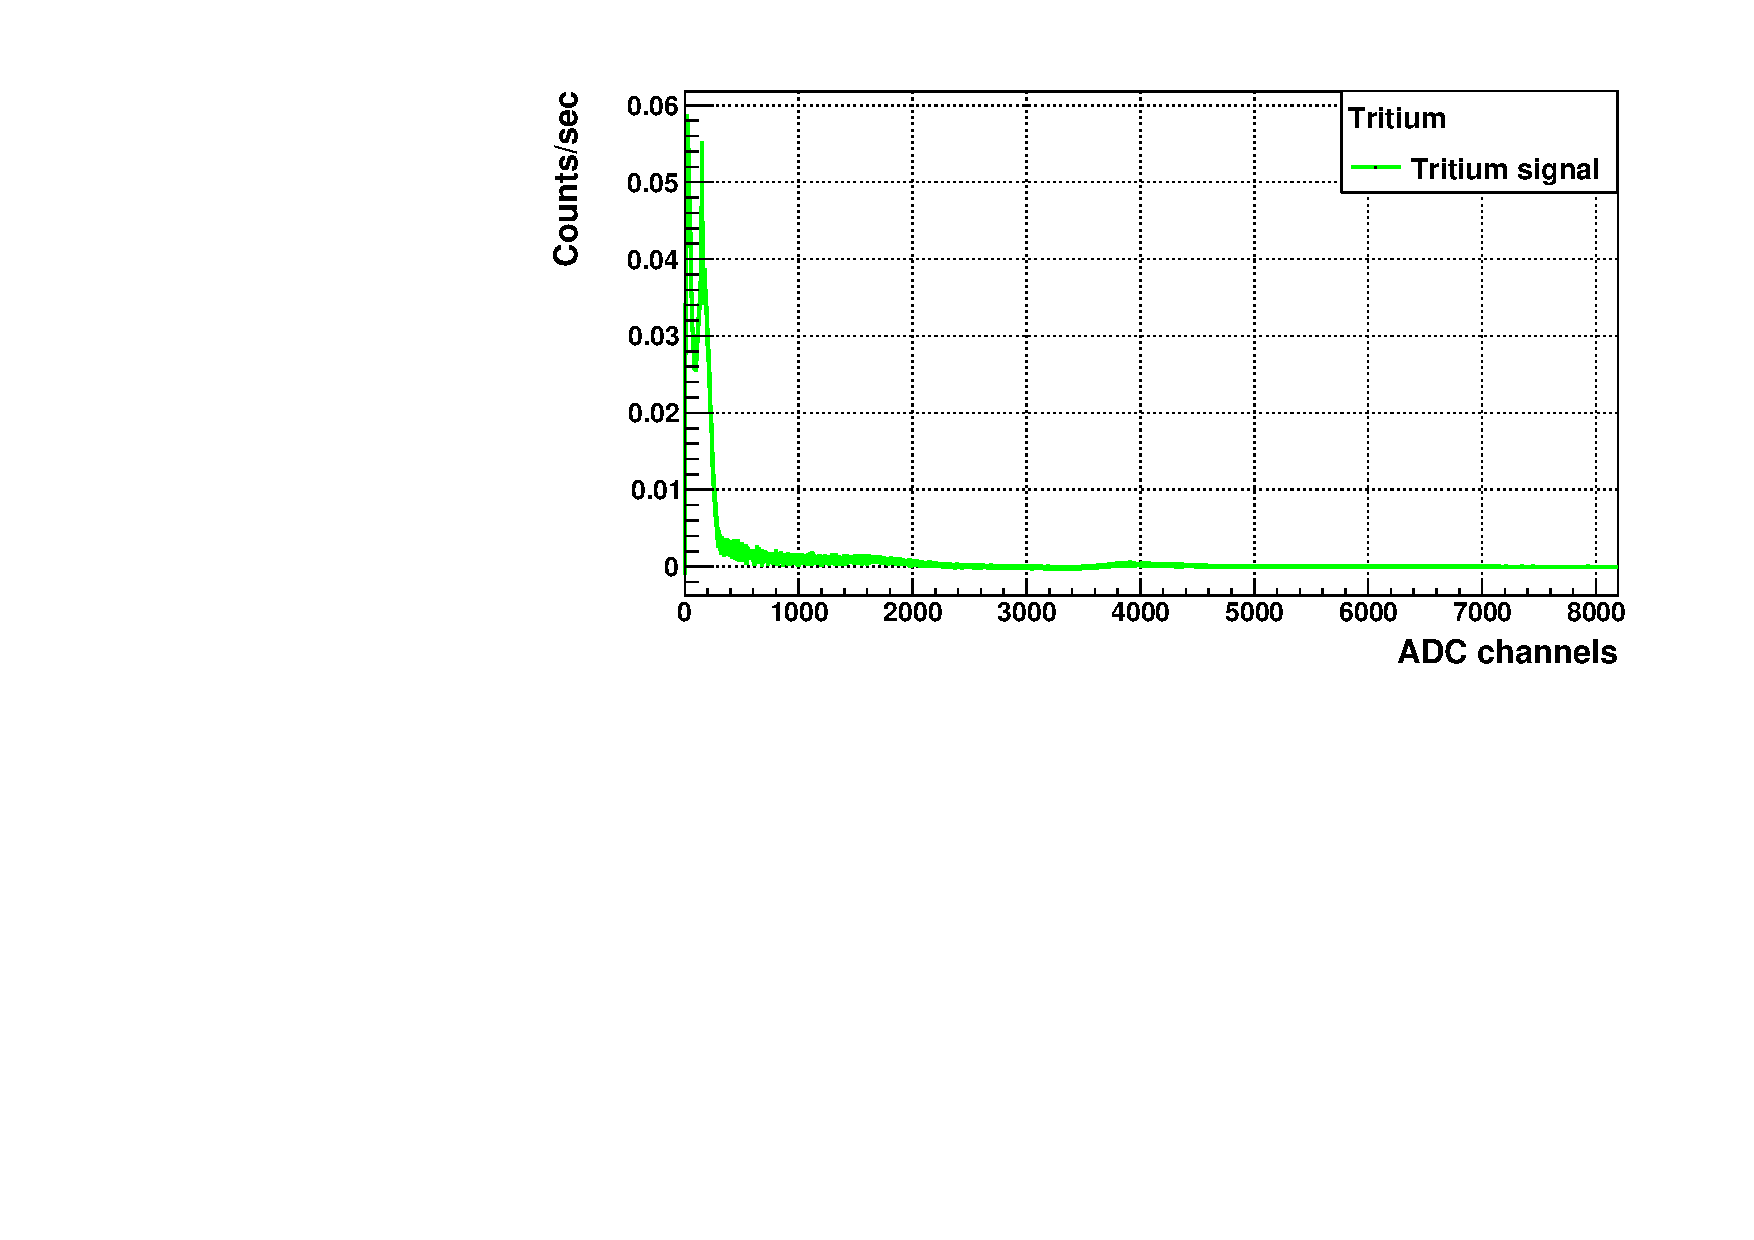
\includegraphics[scale=0.6]{Imagenes/2Efficiency/Net_tritium_signal_real_time.pdf}
\caption{Tritium signal measured in TRITIUM-IFIC 2 prototypes}
\end{figure}


\end{frame}

\begin{frame}
\frametitle{Prototype efficiency measurement}

\begin{figure}[hbtp]
\centering
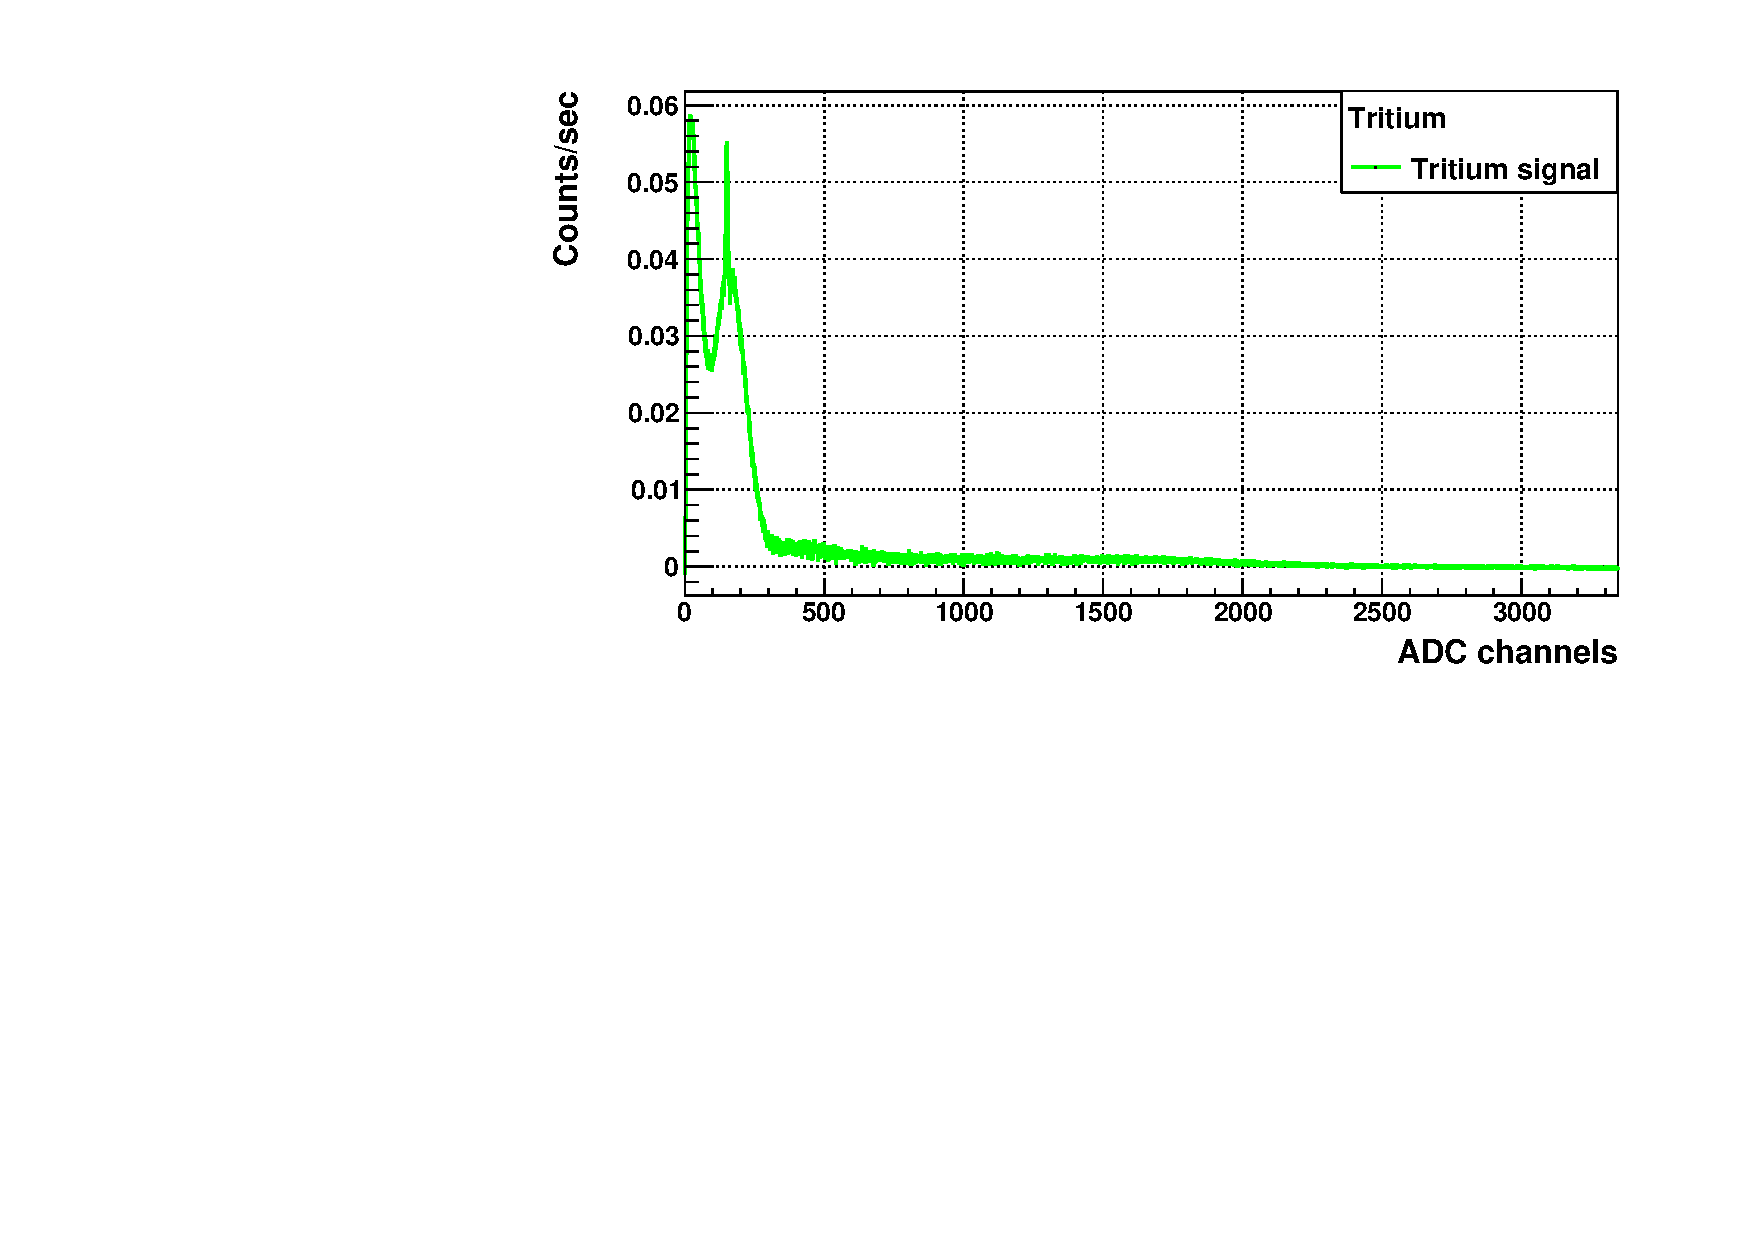
\includegraphics[scale=0.6]{Imagenes/2Efficiency/Net_tritium_signal_real_time_ZOOM.pdf}
\caption{Tritium signal measured in TRITIUM-IFIC 2 prototypes (Zoom 0-4000 channels)}
\end{figure}

\end{frame}

\begin{frame}
\frametitle{Prototype efficiency measurement}

\begin{table}
\begin{tabular}{l | c}
Parameter & Numerical value\\
\hline \hline
Counts/sec (signal) & $19.0522$ \\
Counts/sec (background) & $11.9419$ \\
Counts/sec (Tritium) & $7.11032$ \\
Nominal activity & $10~\kilo\becquerel/\liter$\\
Efficiency & $0.711 ~\frac{c/s}{~\kilo\becquerel/\liter}$ \\
Active area/fiber & $2\pi~\cm^2$\\
Specifical efficiency & $1.415\cdot{}10^{-4}~\frac{c/s}{\cm^2\kilo\becquerel/\liter}$ \\
\end{tabular}

\caption{Results of Tritium-IFIC 2 prototype}
\end{table}

\end{frame}

\begin{frame}
\frametitle{Prototype efficiency measurement}

\begin{table}[htbp]
\begin{center}
\begin{tabular}{l|c|c|c|c}
\hline
 & \parbox{6em}{\centering Efficiency, $\eta_{det}$\\ $(cps/(\kilo\becquerel/\liter))$}  & \parbox{5em}{\centering Surface\\ $F_{sci}$ ($\cm^2$)}  & \parbox{5em}{\centering Specific efficiency\\ $\varepsilon_{det}=\eta_{det}/F_{sci}$} & LDL ($\kilo\becquerel/\liter$)\\
\hline \hline \hline
Muramatsu & $3.85 \cdot 10^{-4}$ & $123$ & $3.13 \cdot 10^{-6}$ & $370$ \\ \hline
Moghissi & $4.5 \cdot 10^{-3}$ & $>424.1$ & $<1.06 \cdot 10^{-5}$ & $37$ \\ \hline
Osborne & $0.012$ & $3000$ & $4 \cdot 10^{-6}$ & $37$ \\ \hline
Singh & $0.041$ & $3000$ & $1.37 \cdot 10^{-5}$ & $<37$ \\ \hline
Hofstetter & $2.22 \cdot 10^{-3}$ & $\sim~100$ & $<2.22 \cdot 10^{-5}$ & $25$ \\ \hline
TRITIUM & $0.711$ & $1600\pi$ & $<1.415 \cdot 10^{-4}$ & $10$ \\ \hline
\end{tabular}

\caption{State-of-the-Art and comparison with our detector}
\end{center}
\end{table}

\end{frame}


\section{Long-term stability of Tritium-IFIC 2 prototypes}
\begin{frame}
\frametitle{Long-term stability of Tritium-IFIC 2 background prototype}

\begin{figure}[hbtp]
\centering
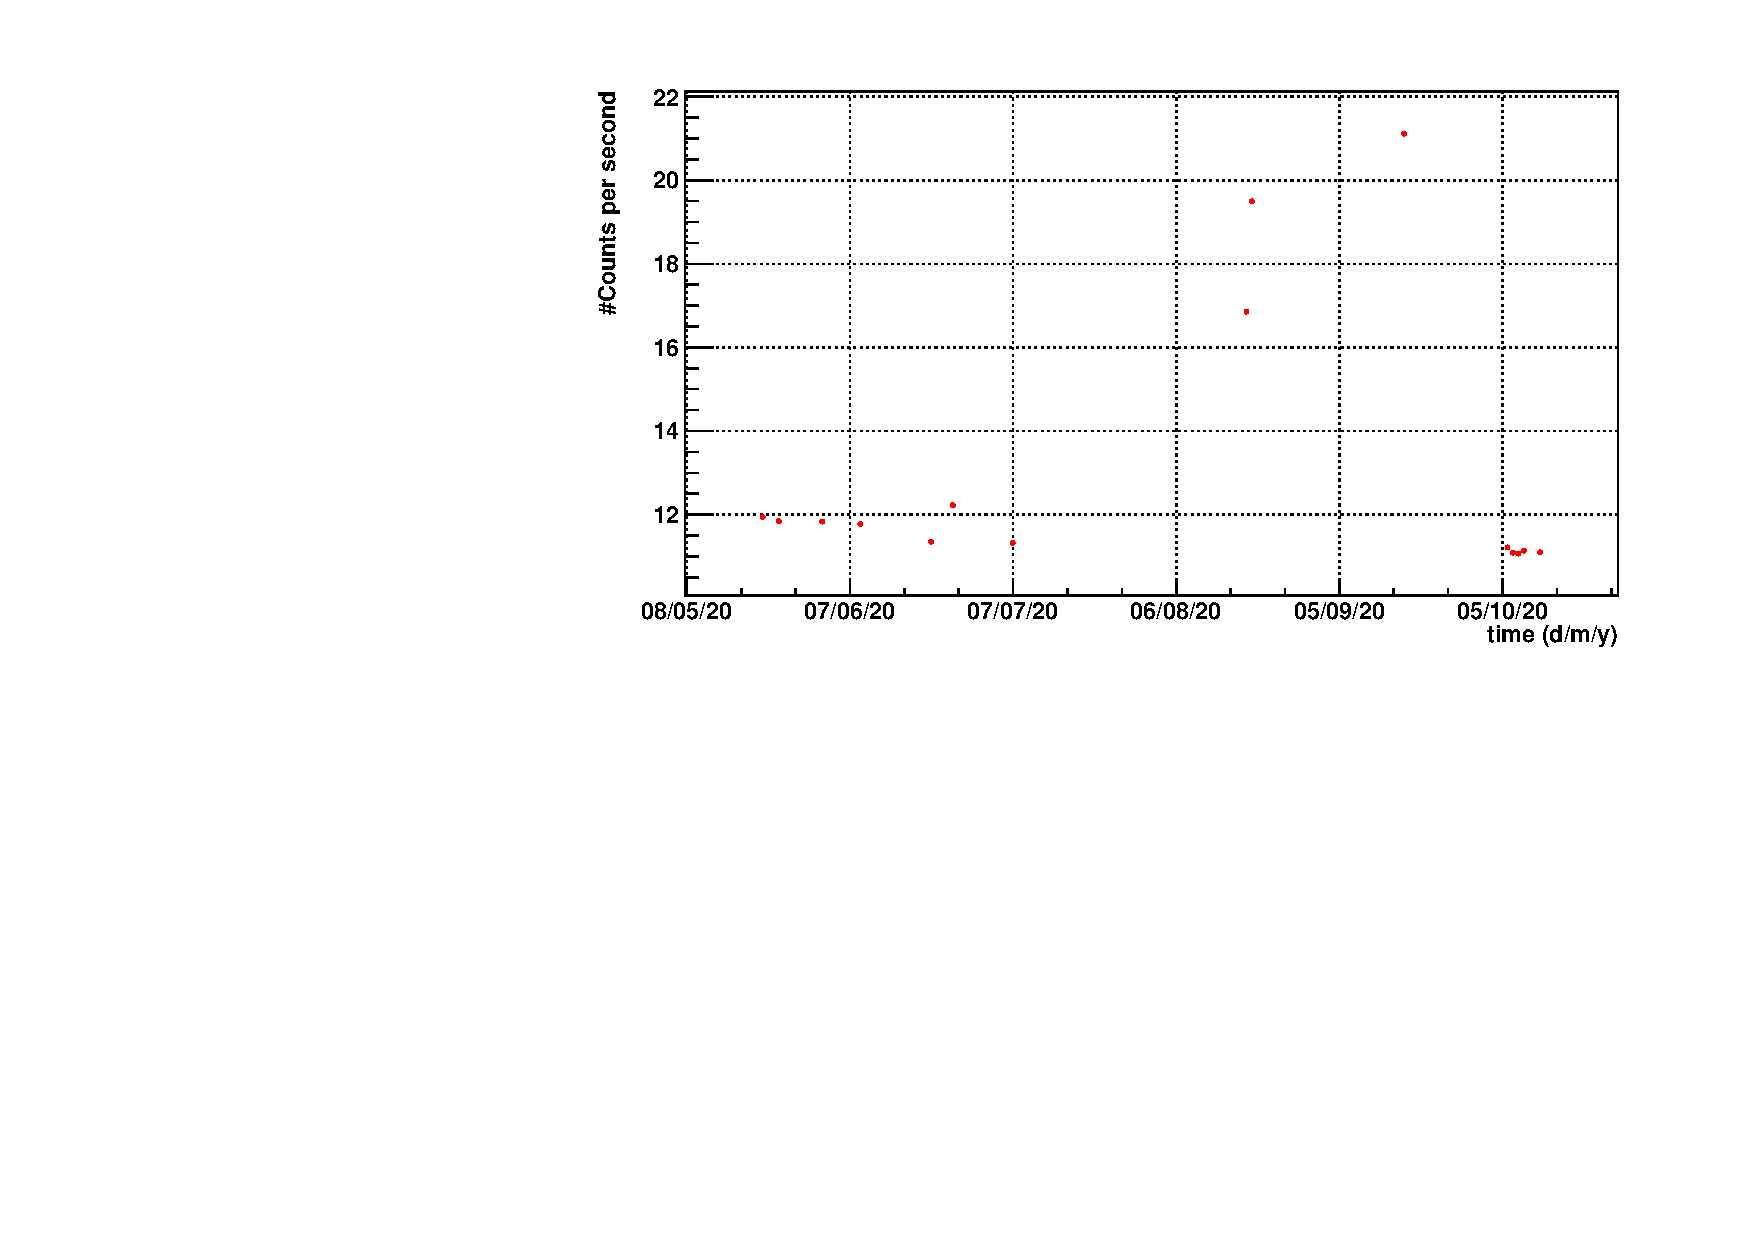
\includegraphics[scale=0.6]{Imagenes/3Long-term_Stability/Monitorizacion_Fondo_rojo.pdf}
\caption{Long-term stability for TRITIUM-IFIC 2 prototype (background).}
\end{figure}

\end{frame}

\begin{frame}
\frametitle{Long-term stability of Tritium-IFIC 2 background prototype}

\begin{figure}[hbtp]
\centering
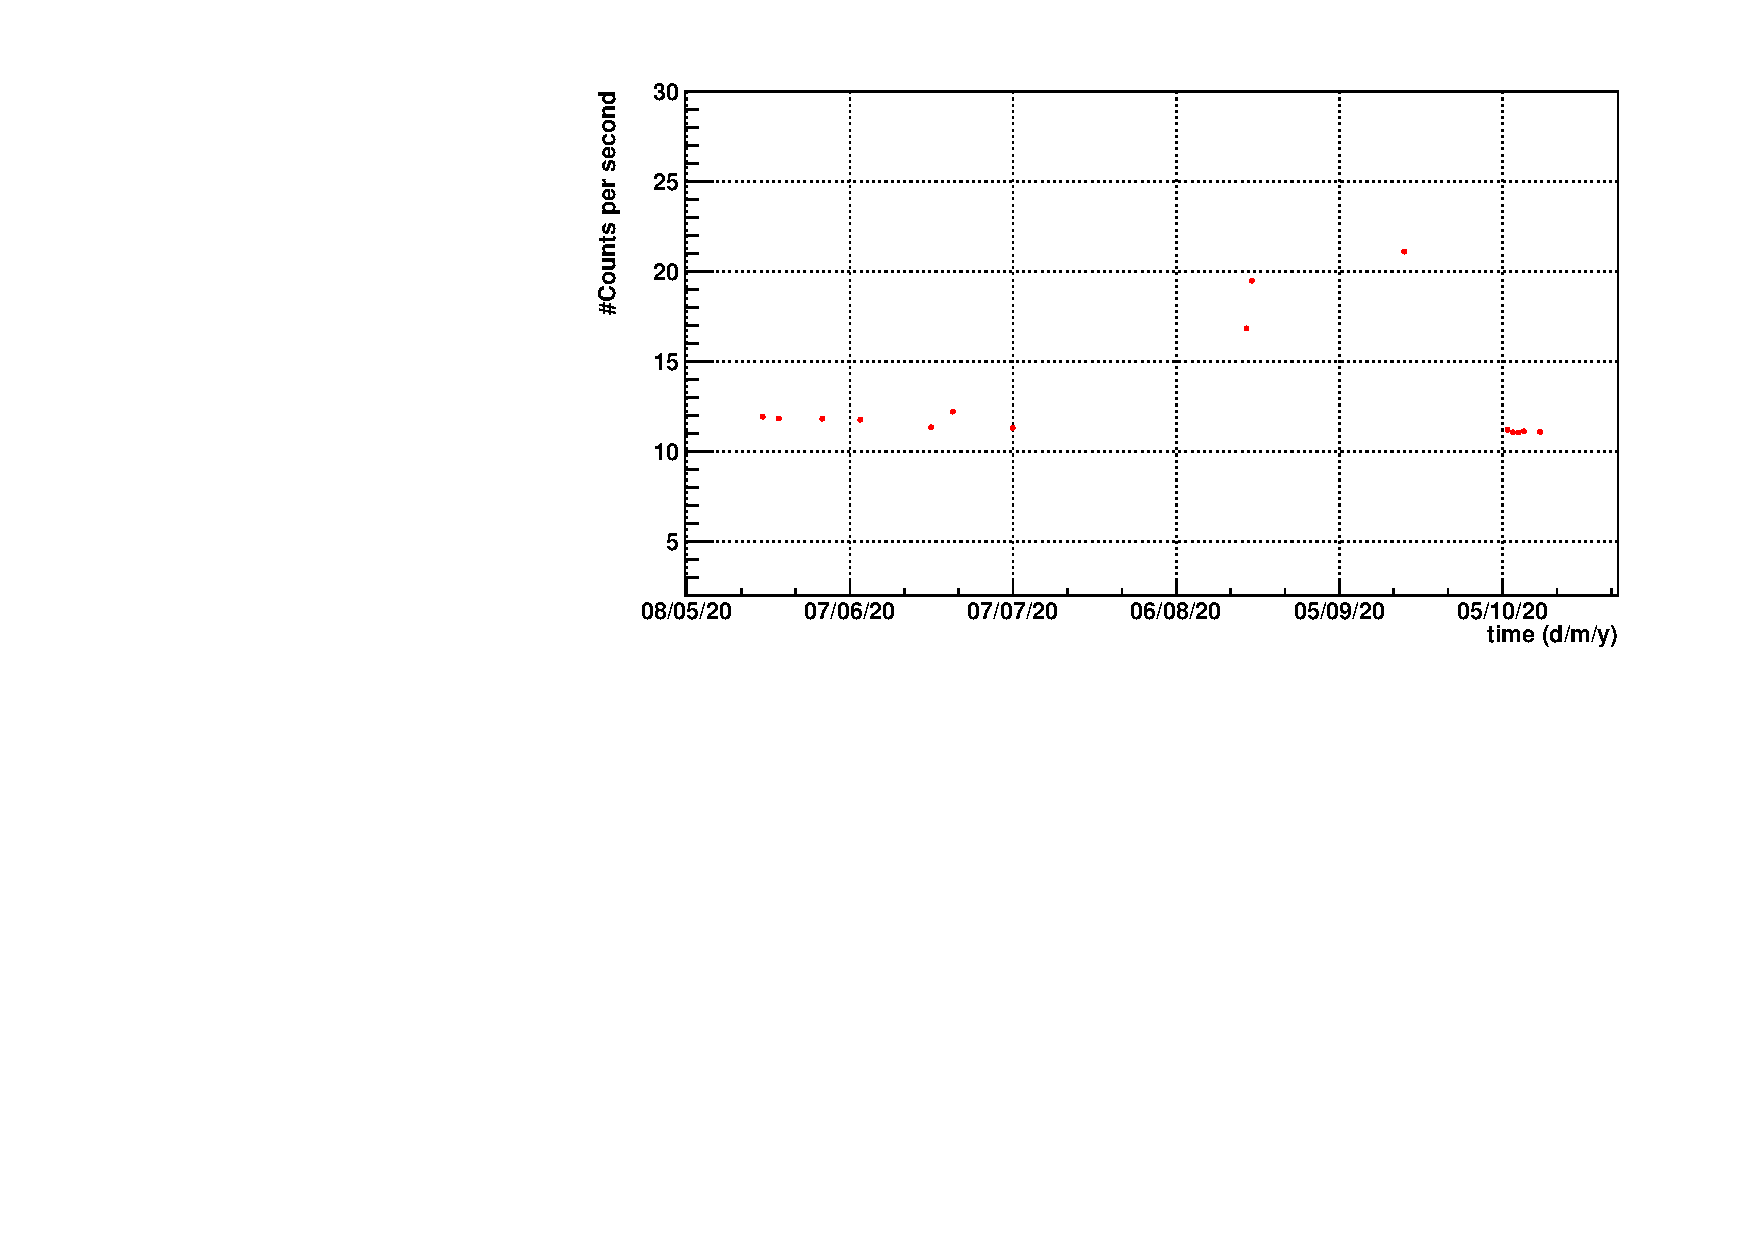
\includegraphics[scale=0.6]{Imagenes/3Long-term_Stability/Monitorizacion_Fondo_rojo_ZOOM.pdf}
\caption{Long-term stability for TRITIUM-IFIC 2 prototype (background). Different ZOOM.}
\end{figure}

\end{frame}

\begin{frame}
\frametitle{Long-term stability of Tritium-IFIC 2 background prototype}

\begin{figure}[hbtp]
\centering
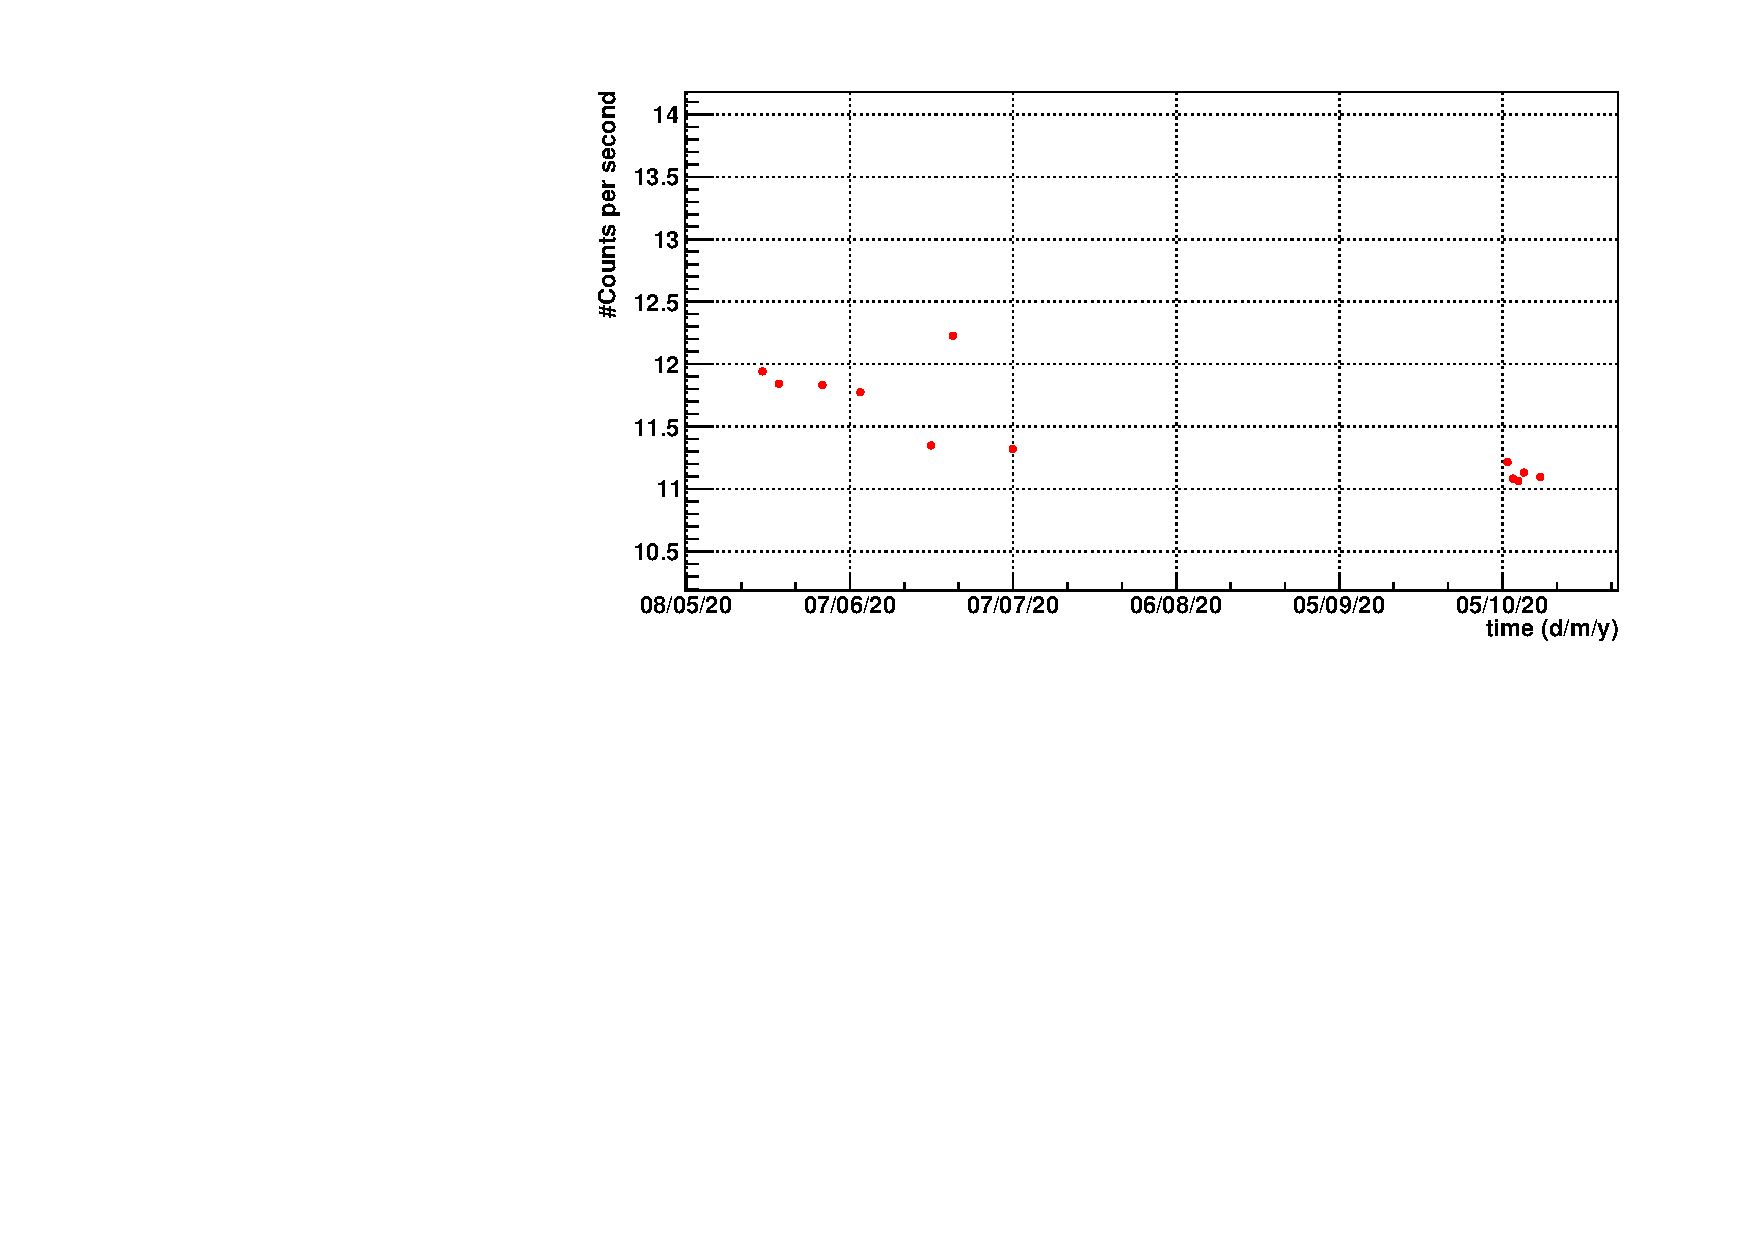
\includegraphics[scale=0.6]{Imagenes/3Long-term_Stability/Monitorizacion_Fondo_rojo_Zoom2.pdf}
\caption{Long-term stability for TRITIUM-IFIC 2 prototype (background). Different ZOOM.}
\end{figure}

\end{frame}

\begin{frame}
\frametitle{Long-term stability of Tritium-IFIC 2 signal prototype}

\begin{figure}[hbtp]
\centering
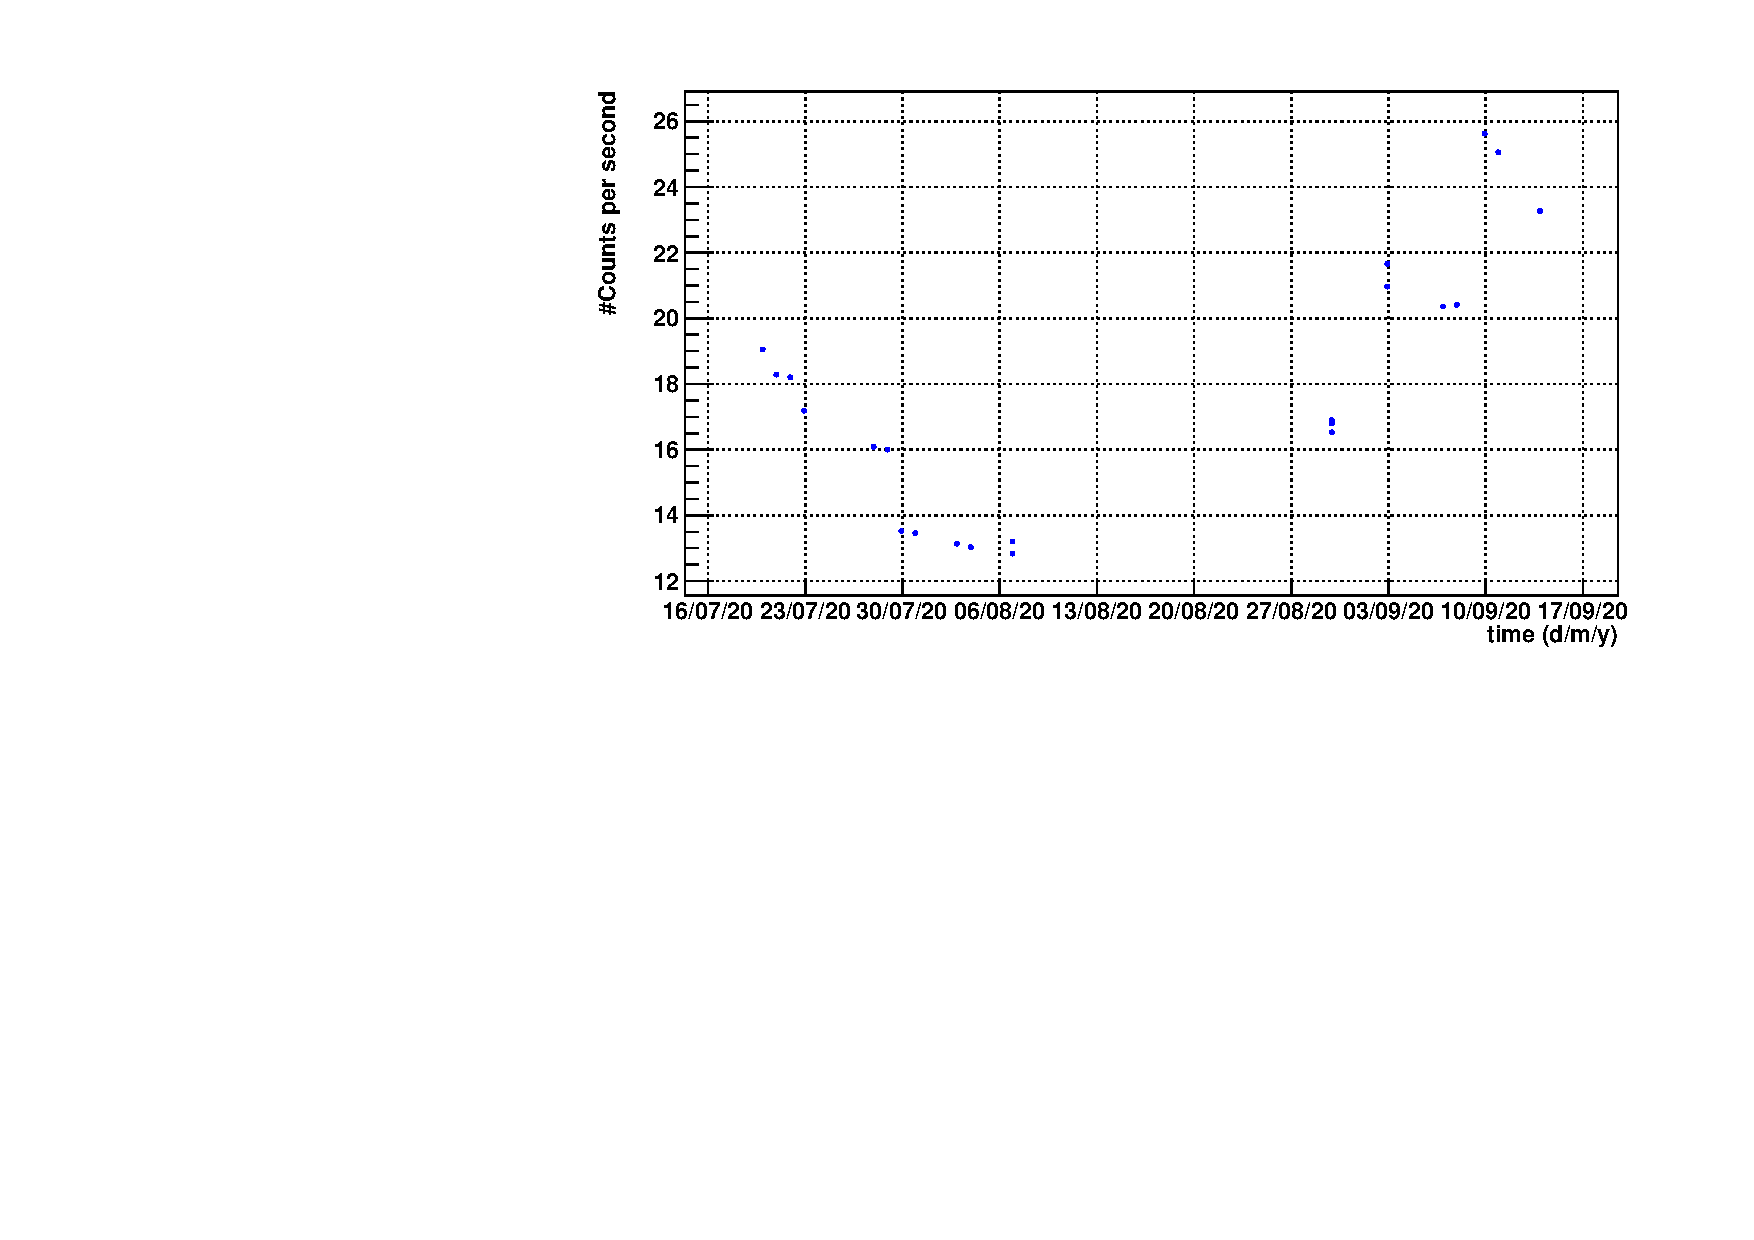
\includegraphics[scale=0.6]{Imagenes/3Long-term_Stability/Monitorizacion_senyal_azul.pdf}
\caption{Long-term stability for TRITIUM-IFIC 2 prototype (signal).}
\end{figure}

\end{frame}

\begin{frame}
\frametitle{Long-term stability of Tritium-IFIC 2 signal prototype}

\begin{figure}[hbtp]
\centering
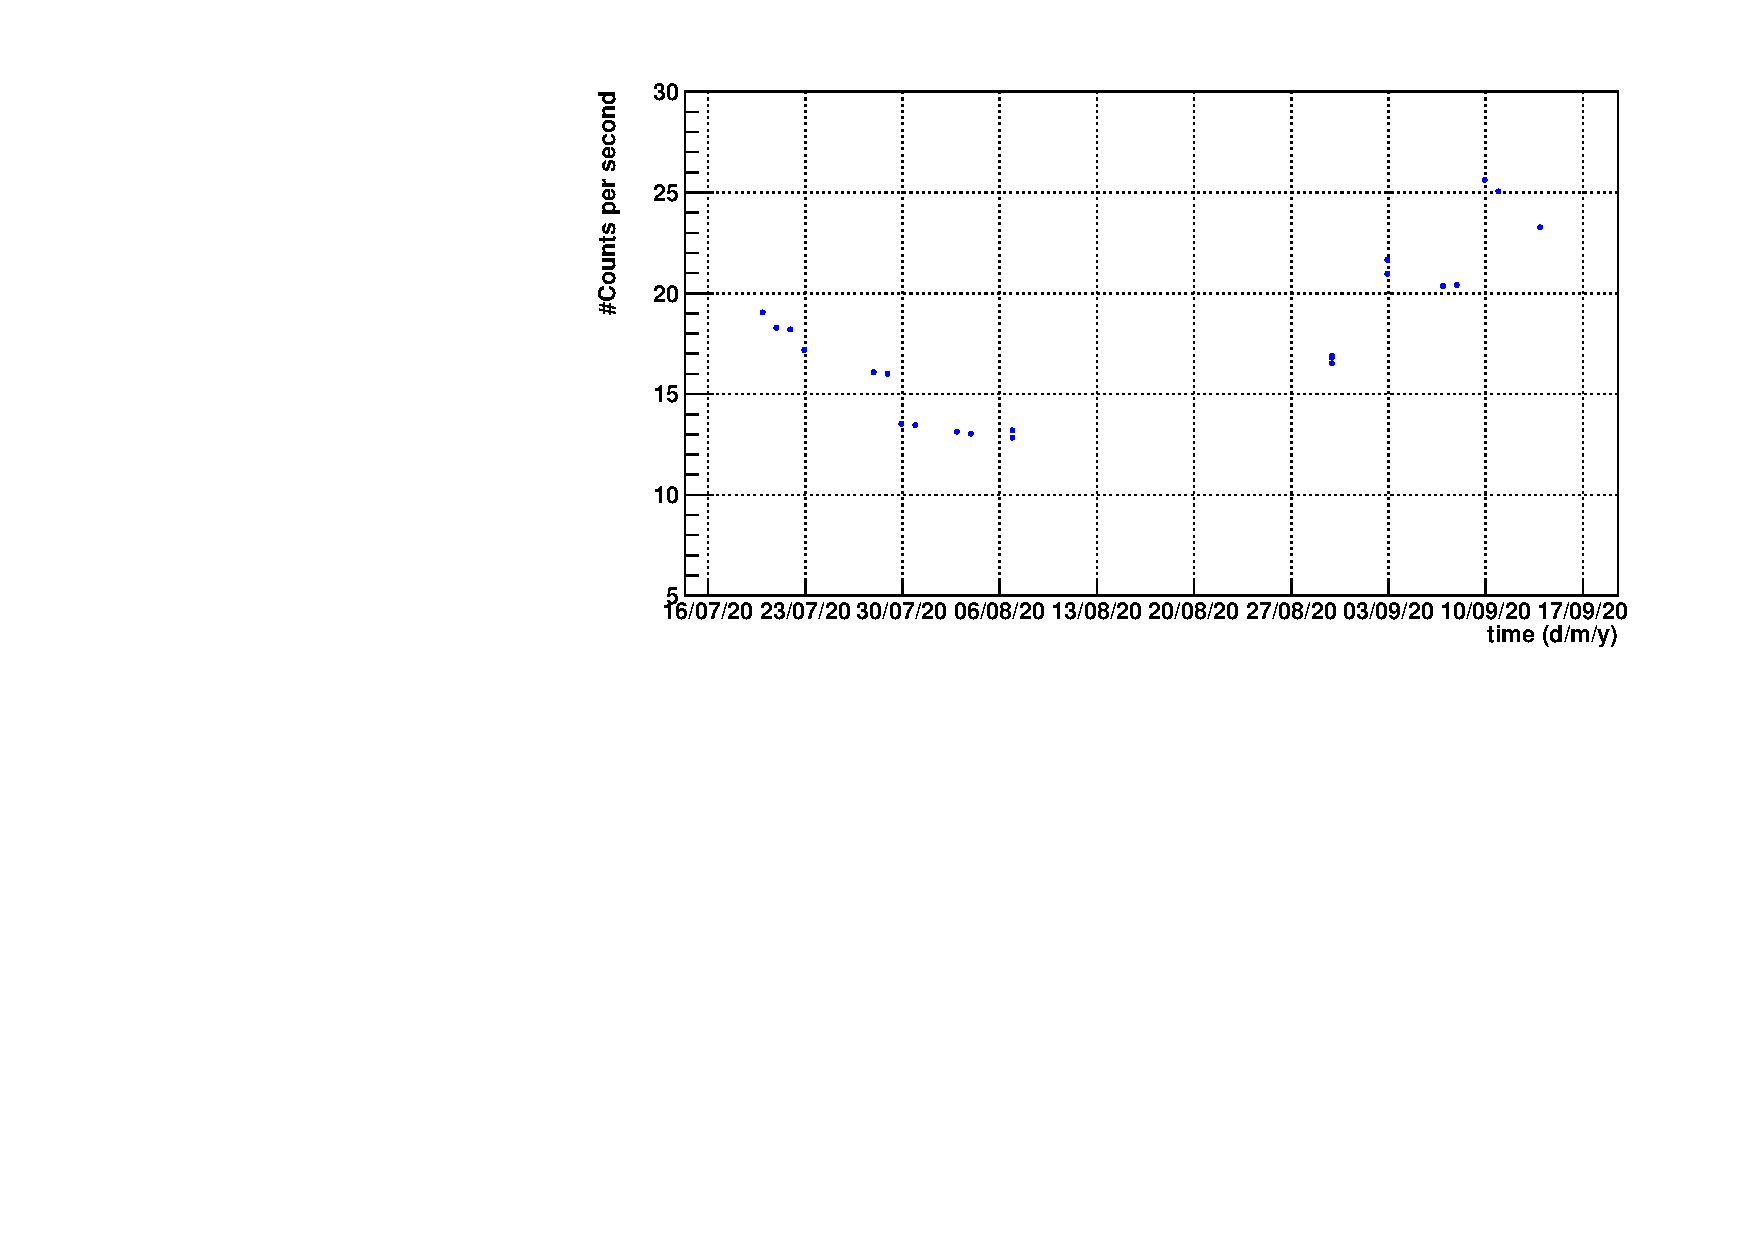
\includegraphics[scale=0.6]{Imagenes/3Long-term_Stability/Monitorizacion_senyal_azul_ZOOM.pdf}
\caption{Long-term stability for TRITIUM-IFIC 2 prototype (signal). Different ZOOM.}
\end{figure}

\end{frame}

\begin{frame}
\frametitle{Long-term stability of Tritium-IFIC 2 signal prototype}

\begin{figure}[hbtp]
\centering
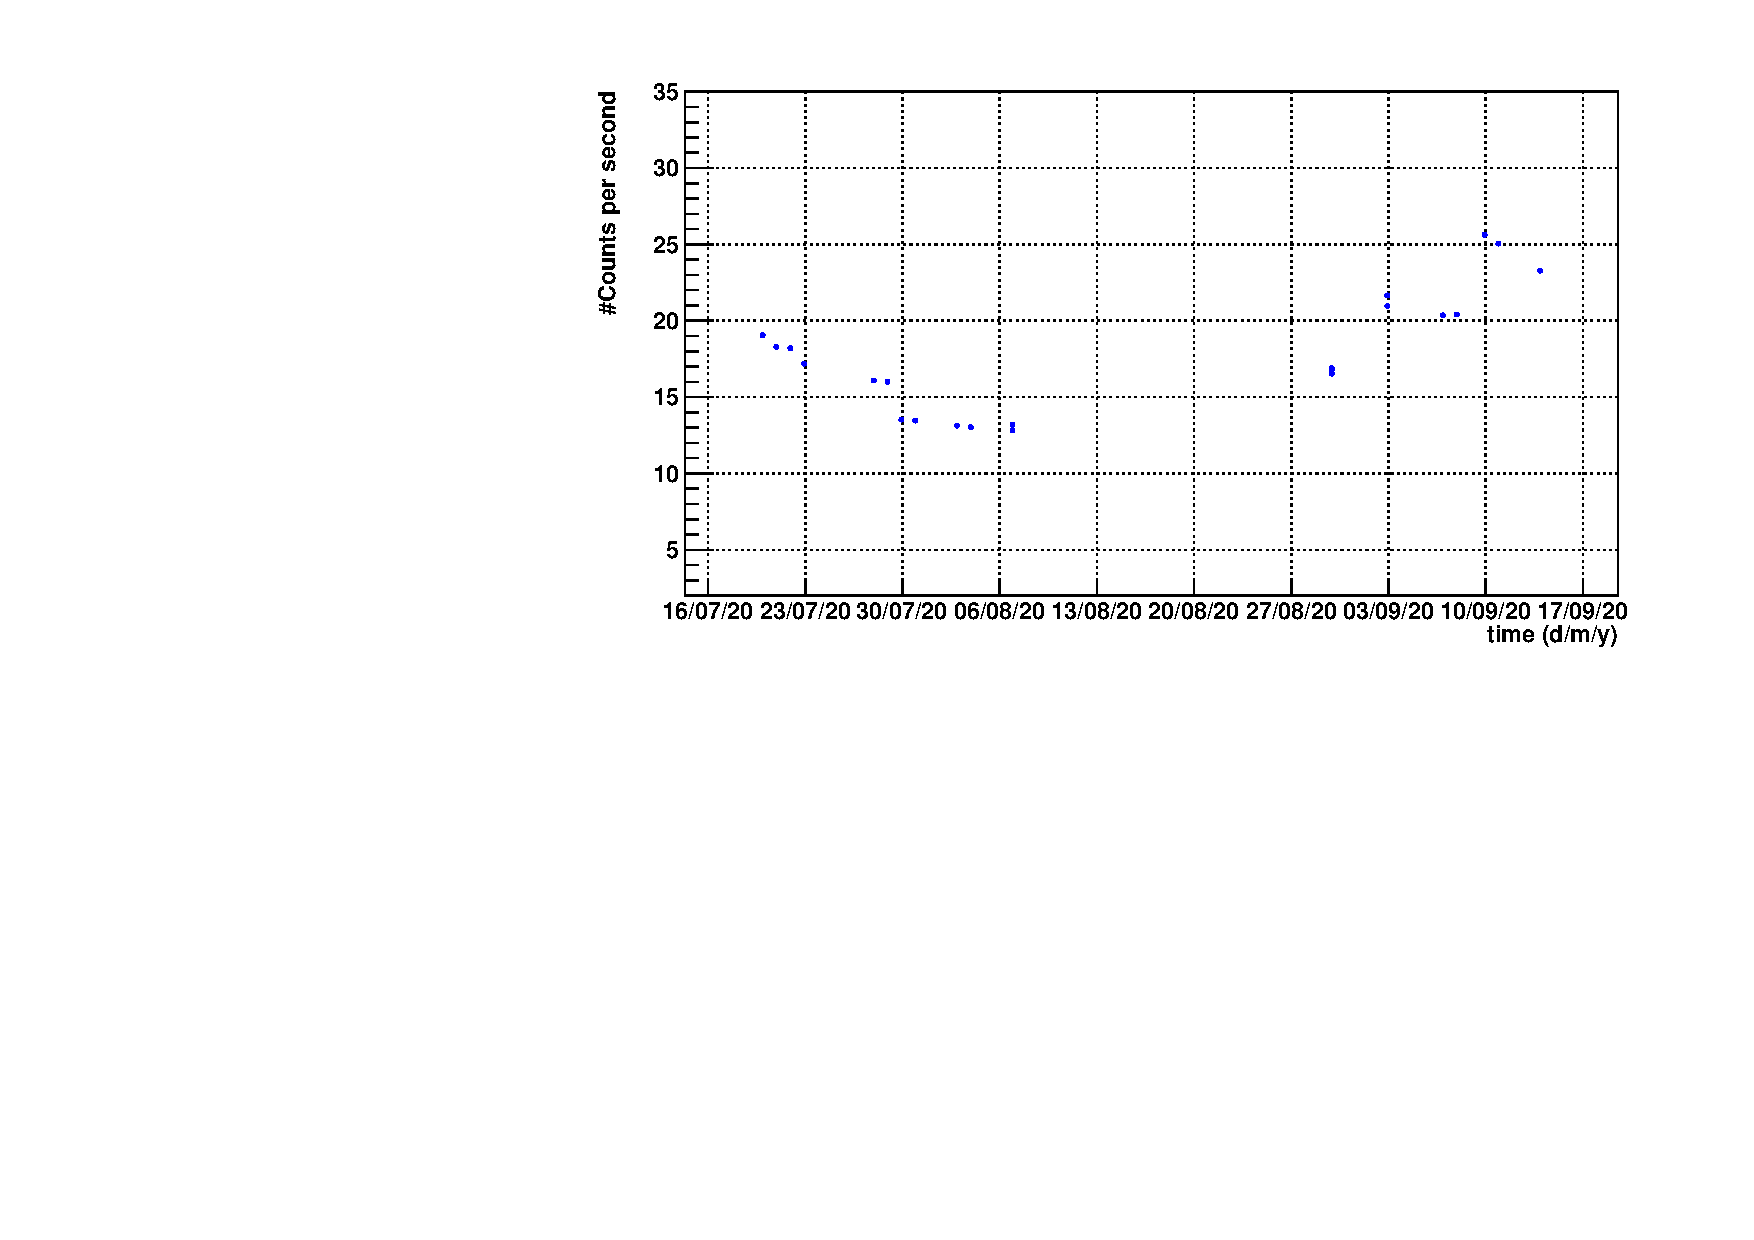
\includegraphics[scale=0.6]{Imagenes/3Long-term_Stability/Monitorizacion_senyal_azul_ZOOM2.pdf}
\caption{Long-term stability for TRITIUM-IFIC 2 prototype (signal).Different ZOOM.}
\end{figure}

\end{frame}


\begin{frame}
\frametitle{Long-term stability of Tritium-IFIC 2 both prototypes}

\begin{figure}[hbtp]
\centering
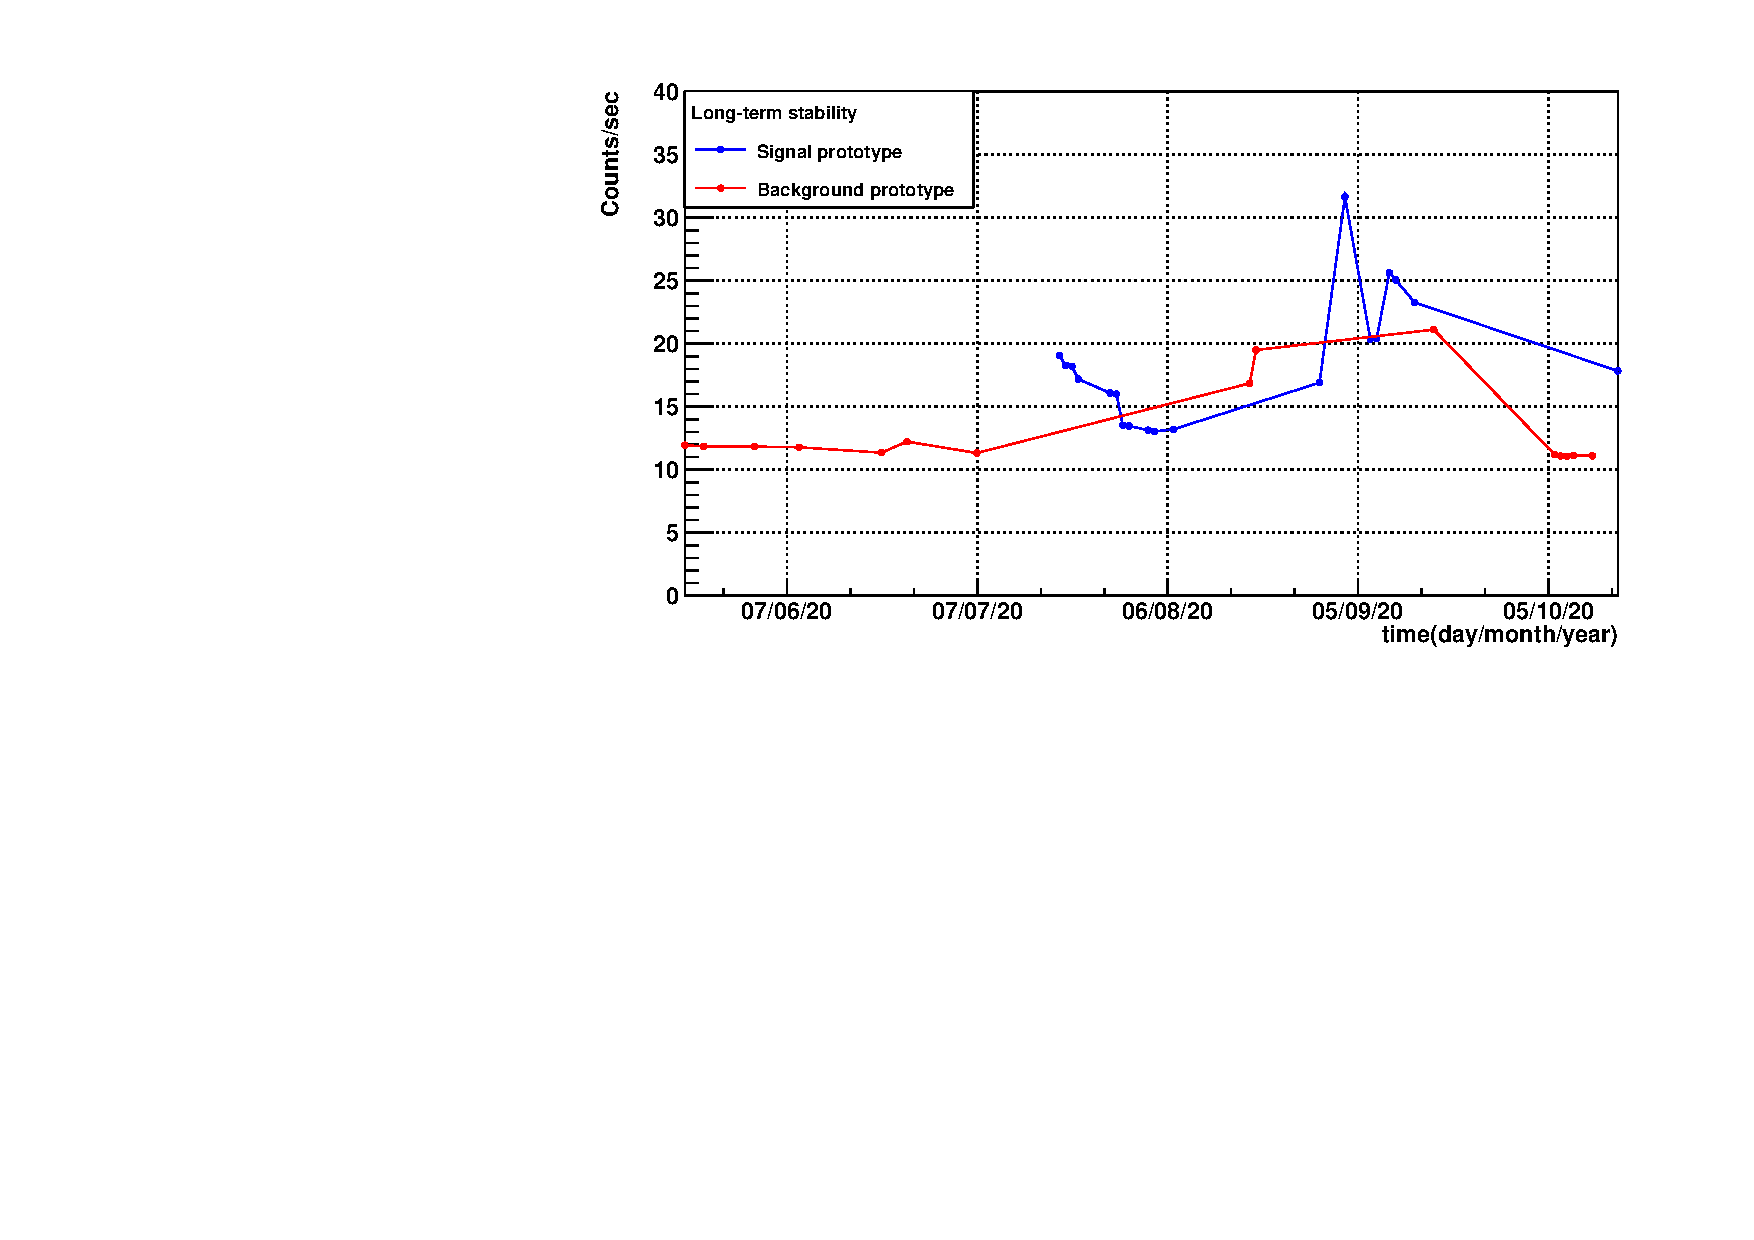
\includegraphics[scale=0.6]{Imagenes/3Long-term_Stability/Both_plots.pdf}
\caption{Long-term stability for TRITIUM-IFIC 2 prototype (signal and background).}
\end{figure}

\end{frame}

\begin{frame}
\frametitle{Long-term stability of Tritium-IFIC 2 both prototypes}

\begin{figure}[hbtp]
\centering
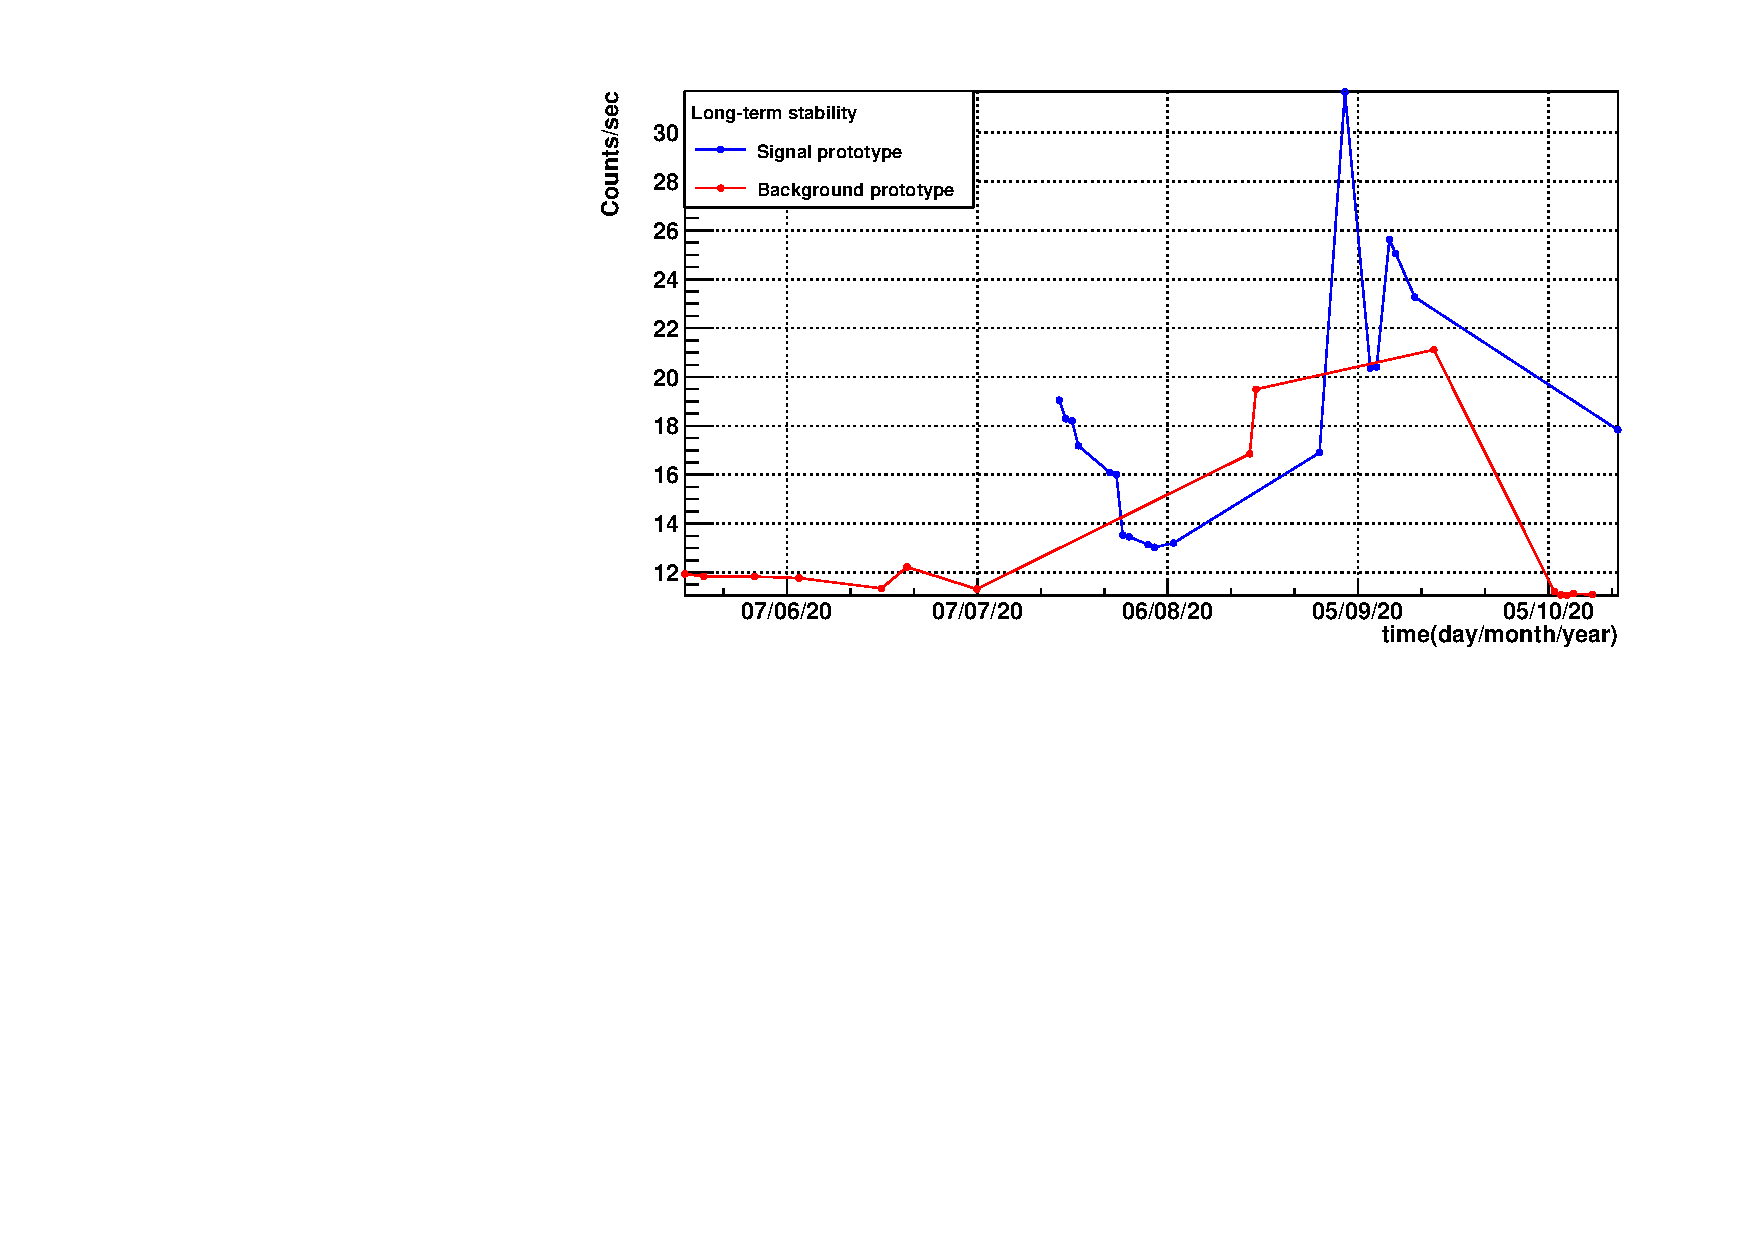
\includegraphics[scale=0.6]{Imagenes/3Long-term_Stability/Both_plots_ZOOM.pdf}
\caption{Long-term stability for TRITIUM-IFIC 2 prototype (signal and background). Different ZOOM}
\end{figure}

\end{frame}

\section{Next step}
\begin{frame}
\frametitle{Next step}

\begin{itemize}
\item{} Measurement of Tritium-IFIC 1:

	\begin{itemize}
	\item{} V=-700V, -750V, -800V 
	\item{} ¿Make sense? $\rightarrow$ Refill $\rightarrow$ Measure again
	\end{itemize}
	
\item{} Refill Tritium IFIC 2 (signal) and measure $\rightarrow$ Friday
\item{} Measure Tritium IFIC 2 (Background and signal) with vetos $\rightarrow$ next week
\item{} Measure Tritium IFIC 2 (signal) with vetos and lead $\rightarrow$ in two weeks
\item{} Build new Tritium IFIC 2 (signal) with less activity $\rightarrow$ ¿$1\kilo\becquerel/\liter$?
\item{} Disassemble the first Tritium-IFIC 2 prototype ($110~\kilo\becquerel/\liter$) to clean it and rebuild it again, probably with new fibers.
\end{itemize}

\end{frame}


\end{document}




